\begin{frame}[fragile]{Soluzione esercizio 3 pt1}

\begin{soluzione}{Soluzione}
\begin{code}
\begin{minted}[linenos]{latex}
\documentclass{article}
\usepackage[a4paper,margin=0cm,landscape]{geometry}
\usepackage{graphicx}
\begin{document}

\begin{figure}
	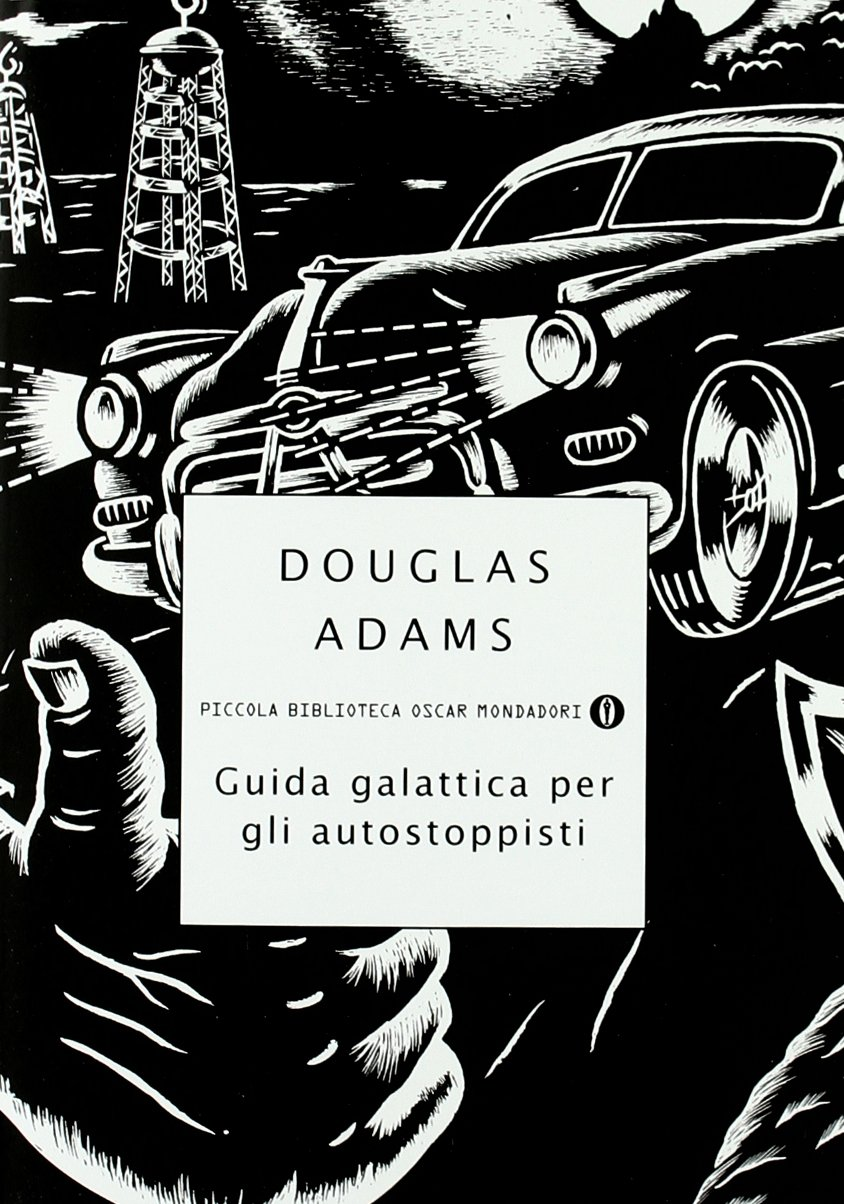
\includegraphics[width=29.6cm, 
	height=20.9cm]{immagine}
\end{figure}

\end{document}
\end{minted}
\end{code}
\end{soluzione}

\end{frame}

\begin{frame}[fragile]{Soluzione esercizio 3 pt2}
Includendo il pacchetto apposito con \mintinline{latex}{\usepackage{atbegshi}}:
\begin{soluzione}{Soluzione Migliore}
	\codedInput{res/examples/soles3.tex}
\end{soluzione}

\end{frame}